\documentclass[12pt,a4paper]{article}

\usepackage{graphicx}
\usepackage{abstract}
\usepackage{hyperref}

\graphicspath{ {./images/} }
\renewcommand{\abstractname}{Timestamps}
\renewcommand{\absleftindent}{}
\renewcommand{\absparindent}{}

\title{CPSC 362 Lecture - poof}
\author{Chris Nutter\thanks{Dedicated to @QuesoGrande}}

% --> Kachow

\begin{document}

\maketitle

\begin{abstract}
    {07:38:48 PM}\\
    Okay so he's talking mainly about the project and how far along people are. 
    People tend to not be incredibly far only a handful of people have created an FSM. 
    He said he is considering adjusting the project depending on our 
    position and understanding of the project.
        \\\\
    07:48:16 PM\\
    Now he is going back to talking about how to implement a DFSM into code. 
    He's sorta doing psuedo-code mentioned below. \emph{Figure 4}
        \\\\
    08:06:36 PM\\
    Taking a break then going to go over non-deterministic FSM (and NFAs).
        \\\\
    08:13:54 PM\\
    You can get 90\% on the project if you document a FSM and diagram it without code. FYI. 
    Basically 90\% for desired output, 100\% for intended FSM.
        \\\\
    08:48:38 PM\\
    Basically he's been making corrolations between video game idles and NFSM. He also mentioned 
    that this will be useful for regexp next week.
        \\\\
    09:11:51 PM\\
    Next time, we are converting NFSM to DFSM. So make sure to understand FSM. lol
\end{abstract}    

\clearpage
\tableofcontents
\clearpage

\section{FSM Recap}
    A finite-state machine (FSM) or finite-state automaton (FSA, plural: automata), 
    finite automaton, or simply a state machine, is a mathematical model of computation. 
    It is an abstract machine that can be in exactly one of a finite number of states at 
    any given time. The FSM can change from one state to another in response to some inputs; 
    the change from one state to another is called a transition.\\\\
    [1] An FSM is defined by a list of its states, its initial state, and the inputs that trigger each transition. 
    Finite-state machines are of two types—deterministic finite-state machines and non-deterministic finite-state machines.\\\\ 
    A deterministic finite-state machine can be constructed equivalent to any non-deterministic one.
        \\\\
    \begin{center}\fbox{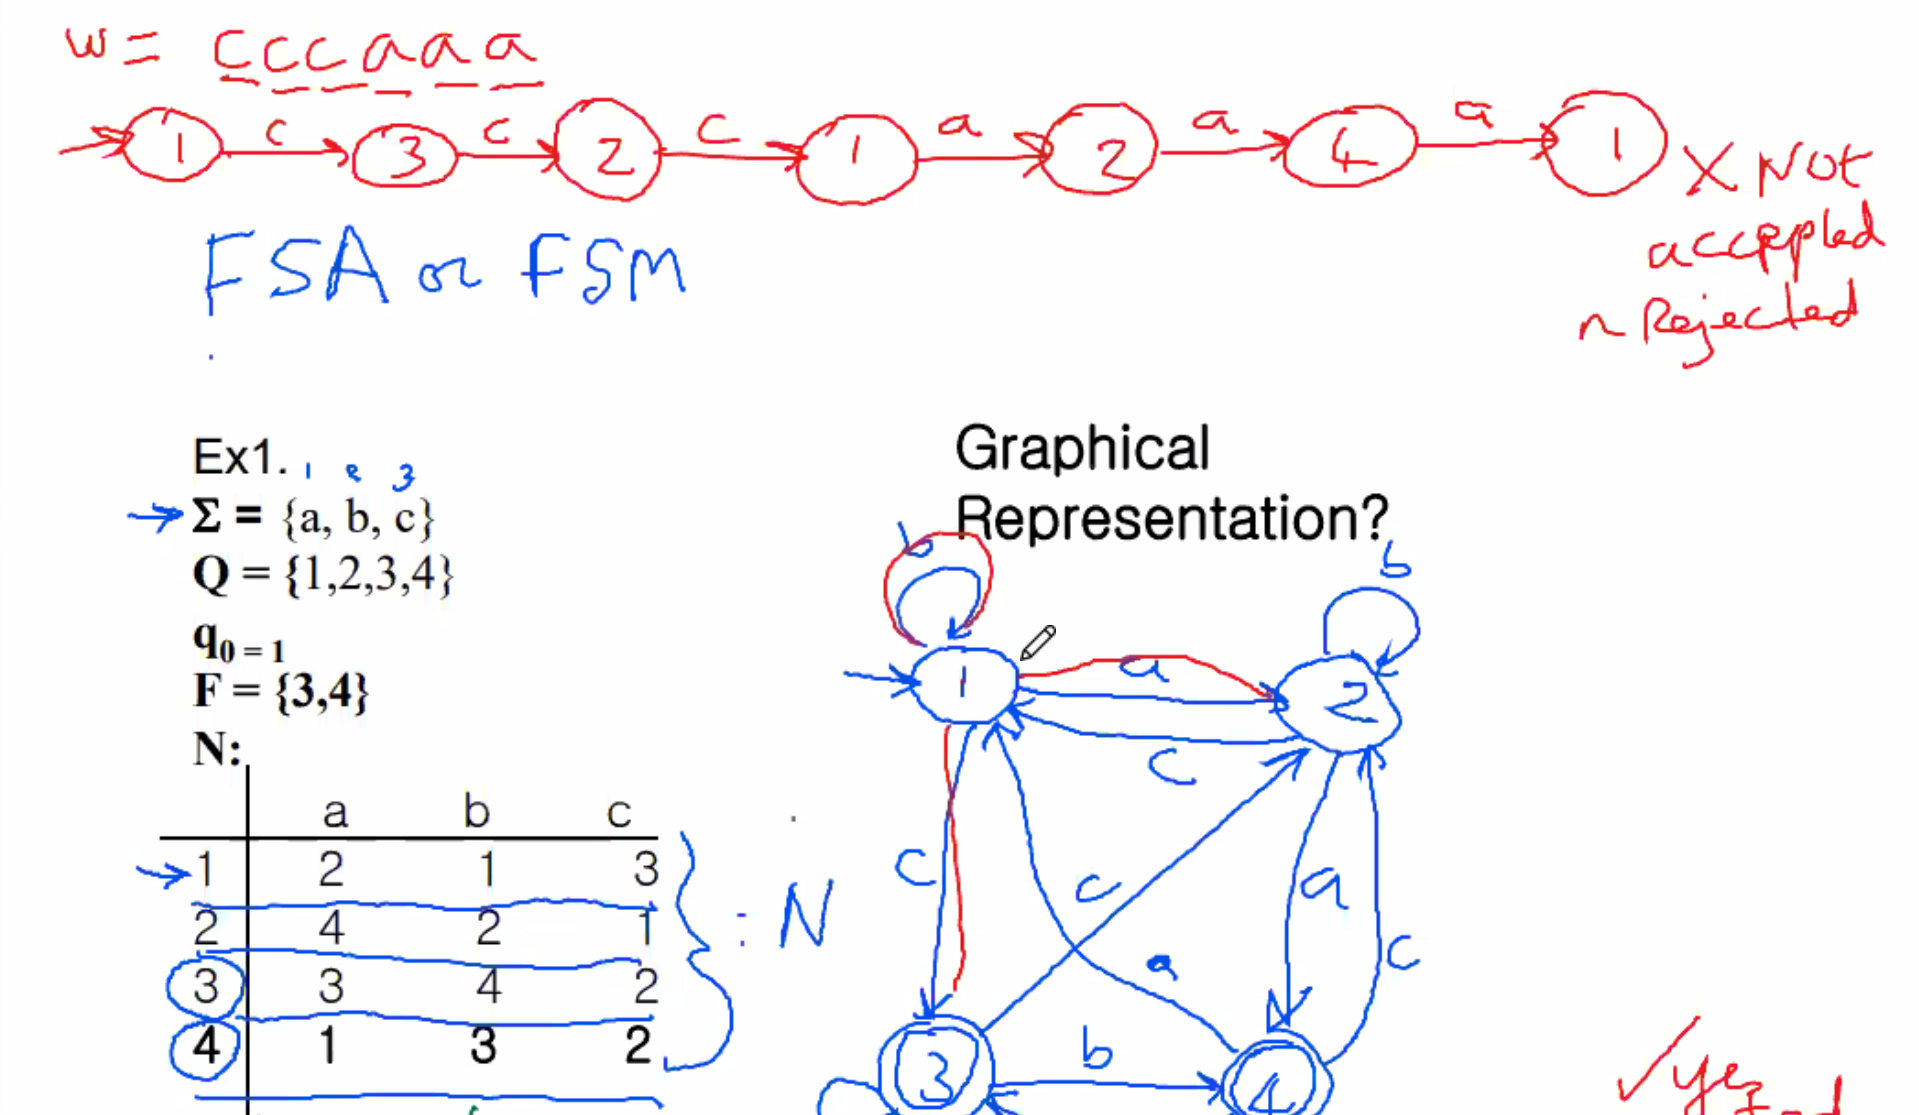
\includegraphics[width=13cm]{fsm.png}}\end{center}

\section{Chapter 2.2 - Deterministic FSM}
    \fbox{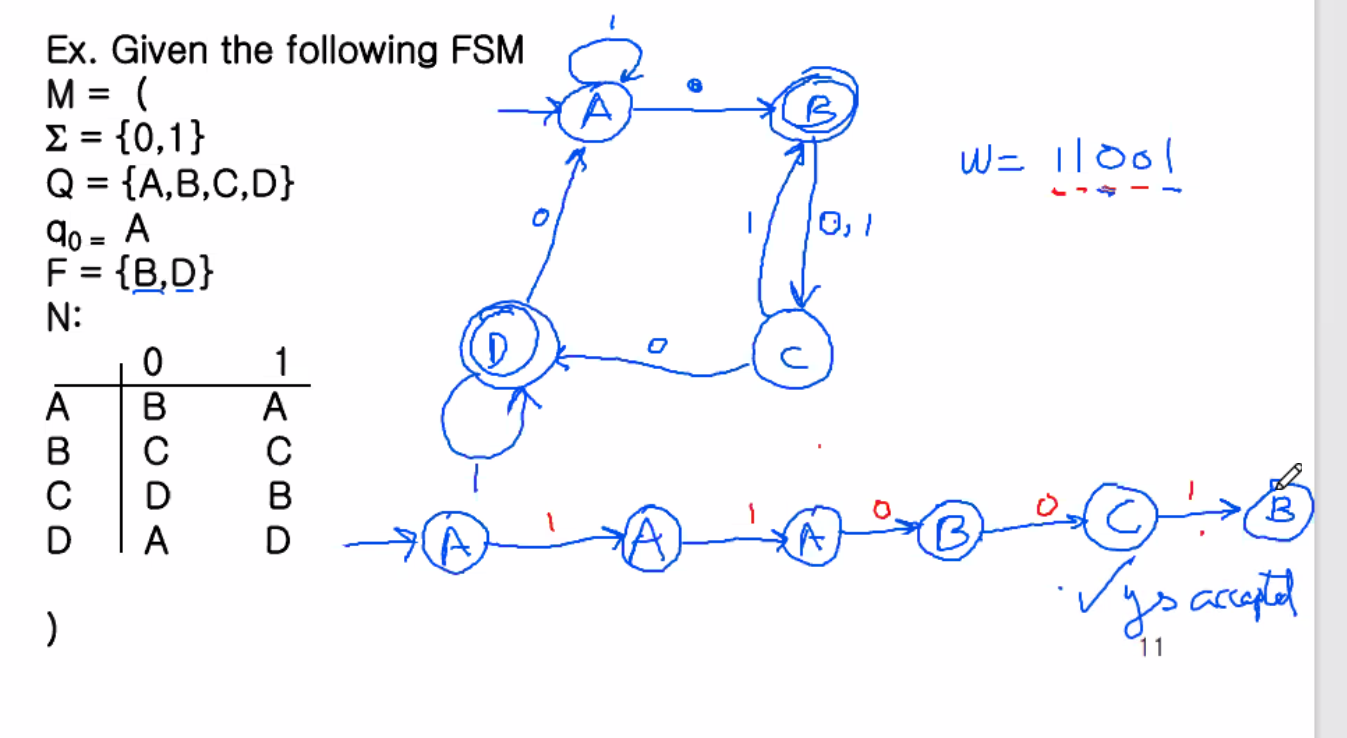
\includegraphics[width=14cm]{example-fsm-problem.png}}
        \\\\
    \fbox{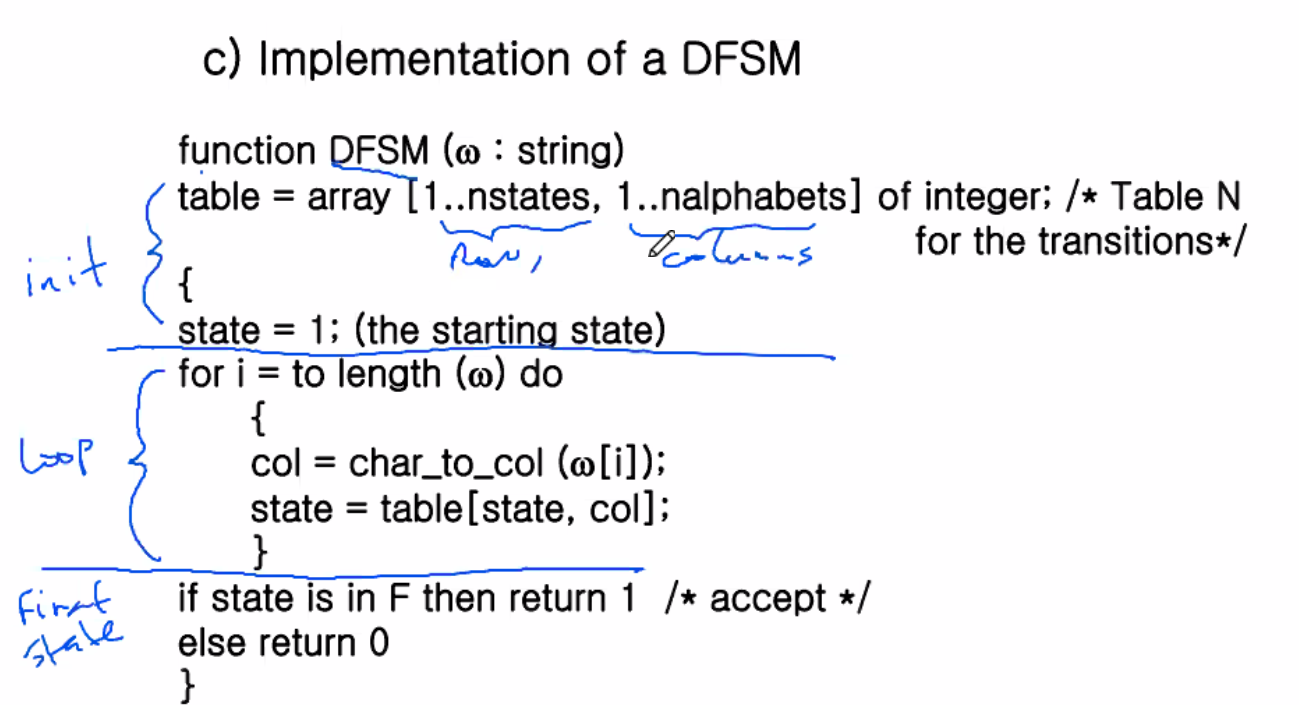
\includegraphics[width=14cm]{implementation-of-dfsm.png}}
        \\\\
    \fbox{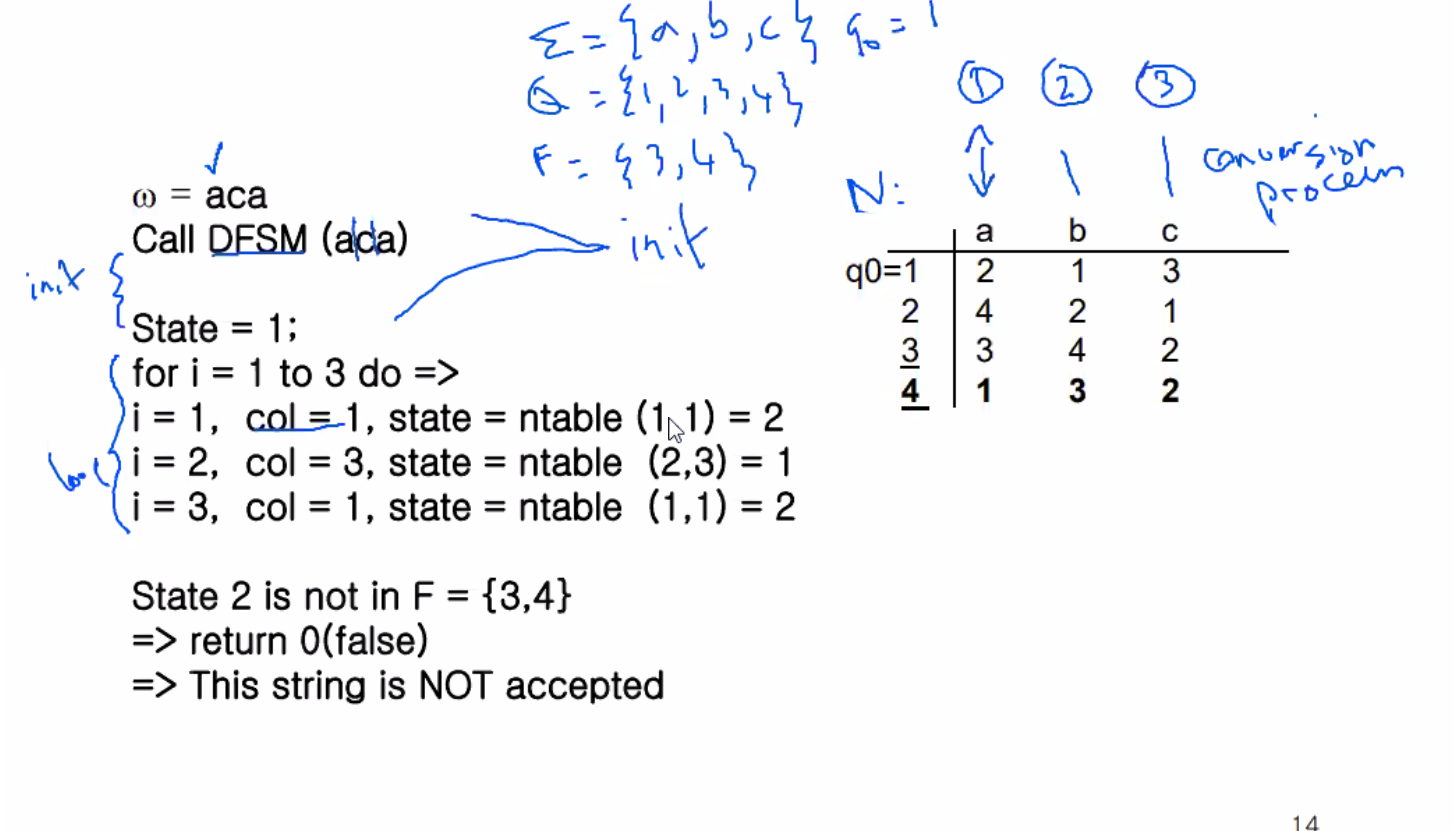
\includegraphics[width=14cm]{implementation-dfsm-w-code.png}}

\begin{center}\line(1,0){250}\end{center}

\section{Chapter 2.3 - Non-Deterministic FSM (NFSM)}
    \fbox{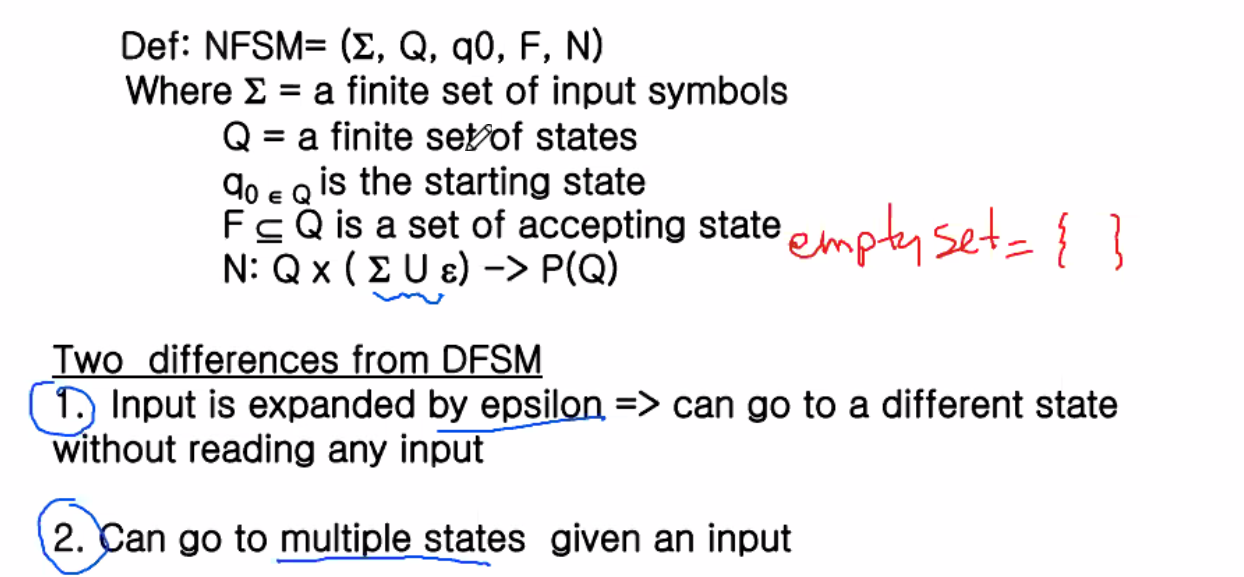
\includegraphics[width=14cm]{nfsm.png}}
        \\\\
    \fbox{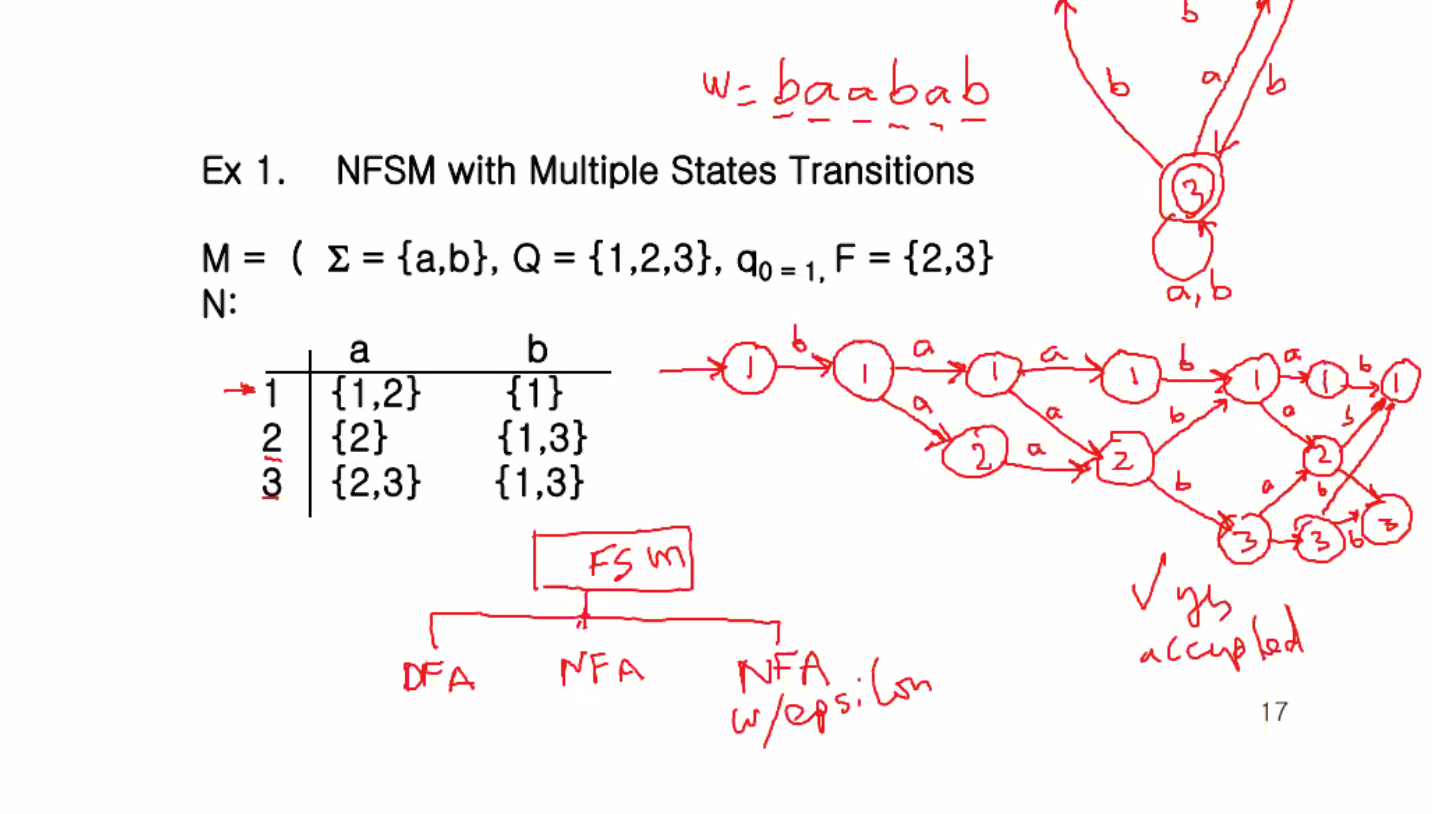
\includegraphics[width=14cm]{ex1-nfsm.png}}
        \\\\
    \fbox{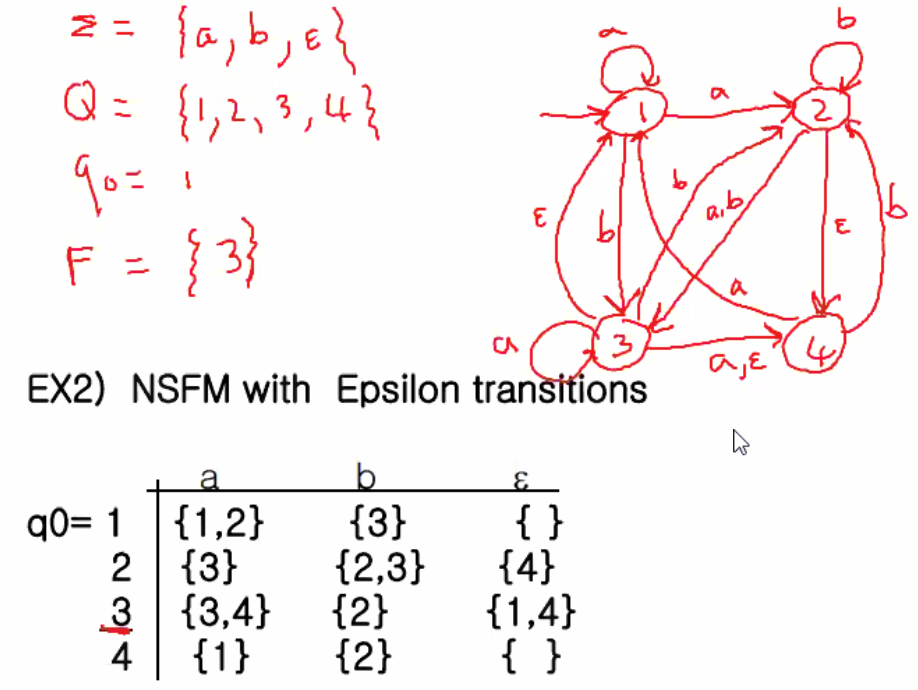
\includegraphics[width=14cm]{nfsm-epsilon.png}}
        \\\\
    \fbox{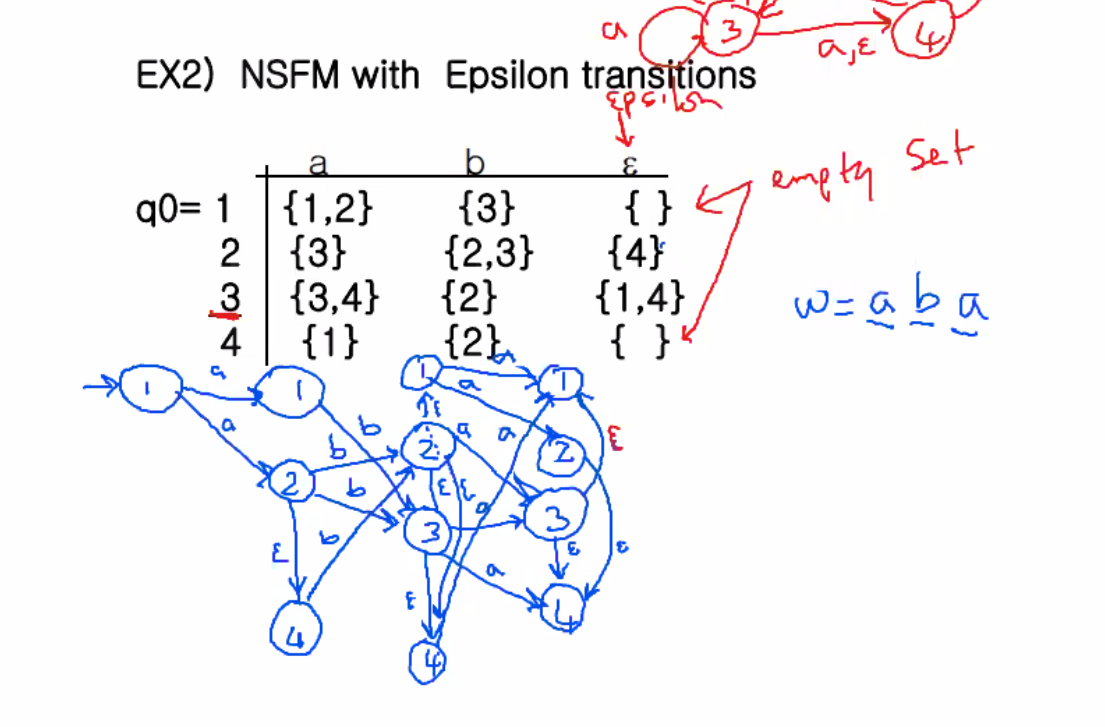
\includegraphics[width=14cm]{ex2-nfsm.png}}

\clearpage

\end{document} 
